\chapter{Features}
\label{chap-2:features}

\begin{table}
  \begin{tabular}{|c|}
    \toprule
    Features \\
    \midrule
    pulls\_count\_open \\
    pulls\_count\_closed \\
    issues\_count\_open \\
    issues\_count\_closed \\
    commits\_count \\
    branches\_count \\
    releases\_count \\
    owner\_type \\
    watchers\_count \\
    forks\_count \\
    stargazers\_count \\
    development\_time \\
    owner\_account\_age \\
    avg\_dev\_account\_age \\
    has\_test \\
    has\_doc \\
    has\_example \\
    has\_readme \\
    owner\_projects\_count \\
    owner\_following \\
    owner\_followers \\
    devs\_followers\_avg \\
    devs\_following\_avg \\
    commits\_by\_dev\_with\_most\_commits \\
    magnetism \\
    stickiness \\
    wealth \\
    last\_commit\_age \\
    \bottomrule
  \end{tabular}
  \caption{Features}
  \label{tab:features}
\end{table}

GitHub repositories are analyzed based on seven different areas.
Each area considers a different aspect of a repository.
Similar works (todo pridat citacie na papiere) analyze repositories in only one extent.
I combined them and gave models (referencia na modely) an overview of a repository qualities across several dimensions. 

The idea is that a repository that is lacking in some of the areas can still excel in others.
Higher number of analyzed features from different categories might result in a better accuracy of classification models.
Some of the models will be able to determine which feature area is better for estimating project survivability than others.
This information might help project owners and contributors to figure out which area their project they should improve on, to increase the chances of a project survival.

These areas and their corresponding sections are:

\begin{itemize}
    \item Popularity \ref{sec:popularity}
    \item Community growth \ref{sec:comm_growth}
    \item Community activity \ref{sec:comm_activity}
    \item Management (zmenit) \ref{sec:management}
    \item Maintenance \ref{sec:maintenance}
    \item Maturity (zmenit) \ref{sec:maturity}
    \item Development rate \ref{sec:development_rate}
\end{itemize}

List of features can be seen in the table \ref{tab:features}.
All of these features are fed as an input for the learning algorithms, they are grouped into areas for the better understandability.

\section{Popularity}
\label{sec:popularity}

Features measured in this category:

\begin{itemize}
    \item stargazers\_count: number of stars
    \item watchers\_count: number of watchers
    \item forks\_count: number of forks
\end{itemize}

While not stated explicitly by GitHub, number of stars\footnote{See \url{https://docs.github.com/en/enterprise-server@2.22/github/getting-started-with-github/github-glossary\#star}} and watchers\footnote{See \url{https://docs.github.com/en/github/getting-started-with-github/be-social\#watching-a-repository}} can be considered as a measure of a project's popularity.

GitHub \emph{stars} are intended to be used primarily to bookmark a repository\footnote{See \url{https://docs.github.com/en/github/getting-started-with-github/saving-repositories-with-stars}}.
Users can also use it as a form of appreciation for the project, it is often used as a proxy for a project popularity \cite{p:1} \cite{p:2} \cite{p:3} \cite{p:6}, even by GitHub\footnote{See \url{https://github.com/trending}}.
Because of ambiguity in terms of user's intentions to \emph{star} a project, I do not consider sufficient to use it as the only popularity metric.

To \emph{watch} a repository, means that the user is interested in getting notified on changes in that repository.
This can indicate a stronger interest than a \emph{star}, as user will receive information about changes in the repository.

Repository might be \emph{forked} when a developer intends to contribute to submit pull requests, fix bugs, add new features and keep copies etc.
These might not be the only reasons to fork a repository, however, high number of forks can still show a high popularity.
Developers are also more likely to fork a project in their preferred programming language \cite{p:10}.

\section{Community growth}
\label{sec:comm_growth}

Features measured in this category:

\begin{itemize}
    \item magnetism
    \item stickiness
\end{itemize}

Magnet projects are those that \textbf{attract a large proportion of new contributors}.
\emph{Magnetism} of a project is the proportion of contributors who made their first contribution in the time period under study who contribute to a given project \cite{p:11}.

In this project, magnetism is computed as a quotient of a number of \emph{new} contributors and a number of \emph{old} contributors.
Old contributors are contributors who committed to the project before a time threshold of two years.
% treba nejak dalej rozvyt tie 2 roky? ze napr. 2 roky pred aktualnym datumom? to by potom trebalo niekde napisat aky je aktualny datum
New contributors, on the other hand, are contributors who committed to the project only after the time threshold.

Figure \ref{fig:magnetism} shows the difference between \emph{new} and \emph{old} contributors, T represents time of the study and A represents time two years before the study.
Developers that contributed to the project before A, the red line, are considered \emph{old} contributors.
Developers that contributed to the project after A, the blue line, are considered \emph{new} contributors.

\begin{figure}
    \centering
    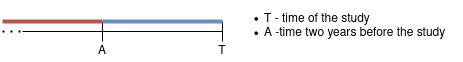
\includegraphics[scale=0.75]{chapters/chapter2/magnetism-new.png}
    \caption{Magnetism}
    \label{fig:magnetism}
\end{figure}

Sticky projects are those where a large proportion of the contributors will keep making contributions in the time period the following and under study \cite{p:11}.
Stickiness in this project is calculated as a quotient of number of contributors that \emph{sticked} and a number of \emph{new} contributors.
Contributors are considered \emph{New} if they commit to the project within past two years.
Contributors that \emph{sticked} are those \emph{new} contributors who still committed to the project within the past year.
It is the proportion of contributors who worked on a given project in the period between one to two years before the study, who also continued to make contributions for the past year before the study.

Figure \ref{fig:stickiness} shows the difference between \emph{new} and \emph{sticked} contributors, T represents time of the study, B represents time two years before the study and A represents time one year before the study.
Developers that contributed to the project between B and A, the red line, are considered \emph{new} contributors.
Developers that contributed to the project between A and T, the blue line, are considered \emph{sticked} contributors.

\begin{figure}
    \centering
    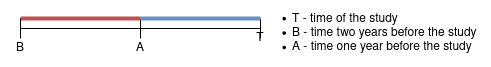
\includegraphics[scale=0.75]{chapters/chapter2/stickiness-new.png}
    \caption{Stickiness}
    \label{fig:stickiness}
\end{figure}

While magnetism metric can indicate how good the project is at attracting new contributors, stickiness can show how good the project is at keeping the new contributors.

\section{Community activity}
\label{sec:comm_activity}

Features measured in this category:

\begin{itemize}
    \item commits\_by\_dev\_with\_most\_commits: number of commits by a contributor with the highest number of commits
    \item devs\_followers\_avg: average number of a repository contributor's followers
    \item devs\_following\_avg: average number of repositories followed by a repository contributor's
\end{itemize}

Small minority of the most active project contributors tend to produce the most activity \cite{top_dev}.
For this reason, it might be useful to consider the most active contributor.
This can be done in several ways.
Measures of activity can be frequency of commits, code addition in commits, message frequency in \emph{Pull requests}\footnote{See \url{https://docs.github.com/en/enterprise-server@2.22/github/getting-started-with-github/github-glossary\#pull-request}} and \emph{Issues}\footnote{See \url{https://docs.github.com/en/enterprise-server@2.22/github/getting-started-with-github/github-glossary\#issue}} and others.
In this project, the most active contributor is selected based on the number of commits.

The average number of followers of developers in the project and the average number of developers/projects followed by them can be seen as an approximation of social relations of project members.
It turns out that project whose developers follow many others are in general more popular.
The effect for developers being followed by many others (i.e. having popular developers in the project) is much weaker.
This discovery results in a practical advice for projects: finding developers engaged in the community is good for the project popularity and can be measured by a simple proxy quantity \cite{p:14}.
Having more popular contributors might improve the project's longevity.

Initially, there was supposed to be another feature in this area, \emph{health}.
In terms of OSS, it is defined as a indicative of three factors of how community activities are performed in a project:

\begin{itemize}
    \item workrate of each contributor
    \item attractiveness of new contributors to a community
    \item active retention of experienced members
\end{itemize}

Labor is measured as community contributions within the projects.
Only source code changes as contributions are considered (i.e., comments made by contributors are ignored) \cite{p:18}.

Although this metric is interesting and potentially very insightful, its computation requires a considerable amount of GitHub API calls\footnote{See \url{https://docs.github.com/en/rest}} to which I have a limited access to.
Compared to most of the other features, it is also resource heavy, which is not suitable for the project of this scale.
For these reasons, I decided to drop this feature, it could be added in the future work.

\section{Management}
\label{sec:management}

Features measured in this category:

\begin{itemize}
    \item owner\_type: type of the repository owner, can be either \emph{organization} or \emph{personal}
    \item owner\_projects\_count: number of repository owner's repositories
    \item owner\_following: number of repositories that the repository owner follows
\end{itemize}

GitHub offers two types of accounts\footnote{See \url{https://docs.github.com/en/github/getting-started-with-github/types-of-github-accounts}}: \emph{personal} and \emph{organization}.
Personal accounts are intended for individual users while organization accounts are for groups of people to collaborate across many projects at once.
Developers are more likely to fork a repository owned by an \emph{organization} type owner \cite{p:10}.

Rationale for the number of project owner's other projects is that the the high number of them might negatively affect the level of maintenance each of them get \cite{p:7}.

Number of repositories followed by the project's owner, the out-degree, tends to be linked with more forks of the project \cite{p:10}.

\section{Maintenance}
\label{sec:maintenance}

Features measured in this category:

\begin{itemize}
    \item has\_test: whether a repository contains a dedicated test code
    \item has\_doc: whether a repository contains a documentation
    \item has\_readme: whether a repository contains a README file
    \item has\_example: whether a repository contains an usage examples
    \item issues\_count\_open: number of \emph{open} issues
    \item issues\_count\_closed: number of \emph{closed} issues
\end{itemize}

Test folder provides the test code for quality assurance, and may help others to test the code they contribute \cite{p:4}.
This makes contributing easier and thus may attract new developers.
Tests are often run periodically in an automated fashion as a part of CI/CD workflow\footnote{See \url{https://www.redhat.com/en/topics/devops/what-is-ci-cd}}.
Such practice greatly improves bug detection and can improve overall project quality.
% todo mozno napisat ze preco tieto stringy?
In this project, a file is considered a test file if it is in a folder named "test, "tests, "t" or "spec".
Presence of a dedicated test folder\footnote{Example \url{https://github.com/jekyll/jekyll}} is shown to be positively correlated with increased number of project forks \cite{p:4}.

It is shown that presence of a proper project documentation is positively associated with the usability improvement of an OSS project \cite{documentation}.
Proper documentation increases understandability and learn-ability of a software.
In this way, it may help with the project maintenance, as new developers are able to join existing community more smoothly.
Project documentation can be provided in several ways.
For smaller projects, it might be sufficient to cover all of the documentation in the \emph{README} file.
Larger projects often require several dedicated documents.
These documents might be incorporated into the GitHub repository\footnote{Example \url{https://github.com/electron/electron}}, or they can reside outside of the repository, for example on the project's web page\footnote{Example \url{https://github.com/facebook/react}}.
Detecting a documentation living outside of the repository would be difficult to do in an automated manner.
% todo mozno dopisat ako som dosiel k tym stringom ktore hladam - vycital som to z papiera 4
This feature looks for a directory named \emph{doc}, \emph{docs}, \emph{document} or \emph{documents}.

As mentioned above, \emph{README}\footnote{See \url{https://docs.github.com/en/github/creating-cloning-and-archiving-repositories/about-readmes}} file may contain a project's documentation.
That is usually the case for very small projects.
It is typically the first thing an user sees in the repository and generally contains information about what the project does, who are its intended users, use cases and so on.
Detecting a \emph{README} file is a straight forward process, we look for a file named \emph{README} in any case and with any extension.

Projects may contain an \emph{examples} folder, containing various usage examples\footnote{Example \url{https://github.com/kubernetes/client-go}}.
Presence of an examples folder may indicate the desire to attract an external attention \cite{p:4}, as these examples are helpful especially for the new users.
In terms of this project, detecting an \emph{examples} folder means searching for the folder named either \emph{example} or \emph{examples}.

The use of these folders suggests a practice of following conventional folder structure in these projects \cite{p:4}.

\emph{GitHub issues}\footnote{See \url{https://docs.github.com/en/enterprise-server@2.20/github/getting-started-with-github/github-glossary\#issue}} can be used for bug reporting, requesting features\footnote{See \url{https://guides.github.com/features/issues/}}, and others.
Creating and commenting on an issue is one of the forms of communication between users of the project and its developers.
It is also often a starting point for new contributors, especially issues labeled as \emph{good first issues} \cite{newcomers}.
Amount of open and closed issues might be a good indicator of two things: project's usage and level of involvement of the developer team.

\section{Maturity}
\label{sec:maturity}

Features measured in this category:

\begin{itemize}
    \item development\_time: time between the first and the latest commit
    \item avg\_dev\_account\_age: average of a repository contributor's accounts age in days
    \item owner\_account\_age: age of repository owner's account in days
    \item owner\_followers: number of a repository owner followers
\end{itemize}

Repository \emph{development time} \label{feature:development_time} is measured in days.
The rationale: projects that are being developed over longer periods of time and are still active have also higher chance of continuing to be active in the future.
It is also an important feature separate suitable repositories for this study from the rest.
Because of many features that require historical data, only projects developed for more than 730 days are being considered.

Note that time between the first and the last commit is not necessarily the same thing as the repository age.
Difference can be demonstrated on the example: repository illustrated in the figure \ref{fig:repo_age} was being actively developed for less than a year.
Other repository, illustrated in the figure \ref{fig:development_age} was being actively developed for almost 2 years, the most recent commit added not very long ago.
Red line in the figures represents development of the project.
Ages of both of these repositories are two years, however, second repository \ref{fig:development_age} clearly has a higher chance of continuing to being actively developed, than the first one \ref{fig:repo_age}.

\begin{figure}
    \centering
    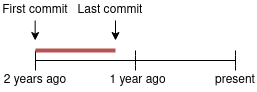
\includegraphics[scale=0.75]{chapters/chapter2/repo_age.png}
    \caption{Shorter development time}
    \label{fig:repo_age}
\end{figure}

\begin{figure}
    \centering
    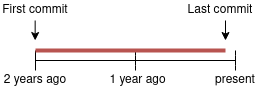
\includegraphics[scale=0.75]{chapters/chapter2/development_age.png}
    \caption{Longer development time}
    \label{fig:development_age}
\end{figure}

Having newer developers in the project is positively correlated with its popularity.
This phenomenon can probably be explained by the fact that programmers may join GitHub in order to contribute to attractive projects \cite{p:14}.
As mentioned in the section \ref{sec:popularity}, gain in popularity can attribute to the project's longevity.

More popular repository owners tend to have older GitHub accounts \cite{p:10}.
Popularity in this context means that repositories of these owners are being forked more often.
Reason for this may be that older project owners (project owners with older GitHub account) are more established in the community or own more projects that are potentially successful.

Related to project owner's popularity is also a number of owner's followers.
More popular owners usually have more followers \cite{p:14}.

\section{Development rate}
\label{sec:development_rate}

Features measured in this category:

\begin{itemize}
    \item commits\_count: number of commits
    \item pulls\_count\_open: number of \emph{open} pull requests
    \item pulls\_count\_closed: number of \emph{closed} pull requests
    \item branches\_count: number of branches
    \item releases\_count: number of releases
    \item wealth: weighted measure based on Pull Requests
    \item last\_commit\_age: age of the last commit in days
\end{itemize}

Features \emph{number of commits}, \emph{number of open pull requests}, \emph{number of branches} and \emph{age of the last commit} are closely related.
To better understand their importance for the study it will be helpful to explain the standard workflow of contribution to a GitHub repository.

\begin{figure}
    \centering
    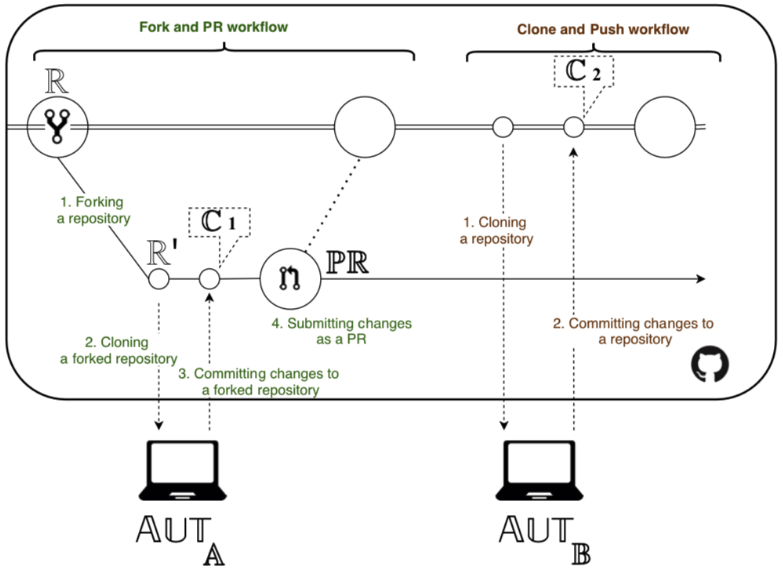
\includegraphics[scale=0.5]{chapters/chapter2/git_workflow.png}
    \caption{Scheme of two types of GitHub workflows \cite{git_workflow}}
    \label{fig:git_workflow}
\end{figure}

Figure \ref{fig:git_workflow} illustrates two types of GitHub contribution workflows: a) Fork and PR workflow and b) Clone and Push workflow.

% todo treba aj toto citovat?
$\mathbb{R}$ denotes a repository, $\mathbb{C}$ set of commit changes and $\mathbb{PR}$ represents a pull request \cite{git_workflow}.

\subsection{Fork and Pull Request (PR) workflow}
\label{sec:fork_pr}

\begin{enumerate}
    \item Fork a repository: A fork is a copy of a repository.
    Forking a repository allows user to freely experiment with changes without affecting the original project.
    Most commonly, forks are used to either propose changes to an existing repository or to use that repository as a starting point for a new project\footnote{See \url{https://docs.github.com/en/github/getting-started-with-github/fork-a-repo}}.
    As shown in the figure \ref{fig:git_workflow}, $\mathbb{AUT_A}$ makes a fork of repository $\mathbb{R}$. We now call this repository $\mathbb{R'}$ \cite{git_workflow}.

    \item Clone a repository: Cloning a repository pulls down a full copy of all the repository data that GitHub has at that point in time, including all versions of every file and folder for the project\footnote{See \url{https://docs.github.com/en/github/creating-cloning-and-archiving-repositories/cloning-a-repository}}.
    This creates a local copy of a remote repository, in which the user can make changes.
    As shown in the figure, $\mathbb{AUT_A}$ clones $\mathbb{R'}$ onto their local computer, become a clone repository $\mathbb{R'_C}$ \cite{git_workflow}.
    
    \item Commit changes to a cloned repository: user can make arbitrary changes to a local copy of a forked repository.
    User can then apply a set of these commit changes $\mathbb{C1}$ to a forked repository $\mathbb{R'_C}$ \cite{git_workflow}.
    
    \item Create a Pull Request (PR): Pull Request enables the user to express an interest in adding their changes to the project.
    Project's owner then decides whether accept those changes or not.
    As shown in the figure \ref{fig:git_workflow}, the pull request $\mathbb{PR}$ contains the set of commit changes $\mathbb{C}$, that will submit to the original repository $\mathbb{R}$, thus completing the workflow \cite{git_workflow}.
\end{enumerate}

\subsection{Clone and Push workflow}
\label{sec:clone_push}

This is a simpler version of Fork and PR workflow \ref{sec:fork_pr}.
Users do not fork a repository $\mathbb{R}$, they only clone it to the local machine.
After making changes $\mathbb{C2}$ in the local version of the repository, users can push them to the original repository $\mathbb{R}$.

\subsection{Features regarding a contribution workflow}

Sections \ref{sec:fork_pr} and \ref{sec:clone_push} demonstrated two basic GitHub contribution workflows.
As we can see, number of commits and Pull Requests closely relates with a development activity of a project.

\emph{Branches} can be created off the base repository branch to safely experiment with changes without a danger of making changes to original files\footnote{See \url{https://docs.github.com/en/desktop/contributing-and-collaborating-using-github-desktop/managing-branches}}.
\emph{Releases} can be create to bundle and deliver iterations of a project to users\footnote{See \url{https://docs.github.com/en/github/administering-a-repository/about-releases}}.
High number of \emph{releases} and \emph{branches} can thus be also one of the indicators of the high development activity.

Wealth in terms of OSS can be defined as the number of completed Pull Requests in month $m$.
To add weight on more recent PRs, we use a weighted measure $PR_m(pr)$ to return the number of months that a PR $pr$ took to close (i.e., $PR_m \leq 1$).
Thus, PRs taking more than a month to complete has less weighting.
% todo zistit ci citovat cely odstaved je ok
Wealth is formally defined as:

% todo trochu som pozmenil oznacenie rovnice - je to ok?
\begin{equation}
    Wealth_m = \sum_{pr \in PRs} \frac{1}{PR_m(pr)}
\end{equation}
